\documentclass{article}

\usepackage[preprint]{neurips_2026}

\usepackage[utf8]{inputenc}
\usepackage[T1]{fontenc}
\usepackage{hyperref}
\usepackage{url}
\usepackage{booktabs}
\usepackage{amsfonts}
\usepackage{amsmath}
\usepackage{amssymb}
\usepackage{nicefrac}
\usepackage{microtype}
\usepackage{xcolor}
\usepackage{graphicx}
\usepackage{enumitem}

\title{Joint-CS: Simultaneous Illumination Normalization and\\ Sparse Image Compression via Unfolded Recovery}

\author{%
  Farhan Sadeek \\
  Thayer School of Engineering\\
  Dartmouth College\\
  Hanover, NH 03755 \\
  \texttt{farhan.sadeek.29@dartmouth.edu} \\
}

\begin{document}


\maketitle


\begin{abstract}
The traditional camera pipeline samples at Shannon--Nyquist rates, compresses to a sparse representation, and only afterwards performs illumination correction on the decoded image. This sequential ordering discards information: sparse recovery applied to a signal whose dynamic range is dominated by an unknown multiplicative illumination field has weaker recovery guarantees than the same recovery applied to the underlying reflectance. We formulate \emph{Joint-CS}, a single inverse problem in the joint variables of DCT-domain reflectance coefficients and a smooth per-column illumination field, and solve it by block-coordinate alternation between a learned-iterative-shrinkage step on the coefficients and a closed-form ridge step on the illumination. Across four experiments---an empirical Donoho--Tanner phase transition, rate-distortion on a natural image, a deep-unfolded LISTA solver, and an ablation against a sequential CS-then-illumination-correct baseline---we find that the joint formulation outperforms the sequential one by 1.4--2.9~dB PSNR across measurement rates under an $8\times$ horizontal illumination gradient, and that a $K{=}10$ unrolled LISTA matches what FISTA needs $22$ iterations to reach.
\end{abstract}


\section{Introduction}
\label{sec:intro}

Modern imaging pipelines acquire $N$ pixels via Nyquist sampling, then immediately throw most of that information away: a typical JPEG keeps only $\sim 5$--$10\%$ of the DCT coefficients above the quantization floor, and the image signal processor (ISP) further reshapes the data through demosaicing, tone-mapping, and white-balance correction. Compressed sensing (CS) reverses this order. If the signal $\boldsymbol{x}$ is $S$-sparse in some basis $\boldsymbol{\Psi}$, then $M \ll N$ random linear measurements $\boldsymbol{y} = \boldsymbol{A}\boldsymbol{x} + \boldsymbol{w}$ suffice to recover $\boldsymbol{x}$ exactly (up to noise) by solving an $\ell_1$ minimization, provided $\boldsymbol{A}$ obeys the restricted isometry property~\citep{candes2006stable,donoho2006compressed}.

CS has been extensively studied for compression. It has been less extensively studied as an integrated stage of a RAW image-signal pipeline. The crux of the issue is that a RAW sensor measures the product
\begin{equation}
  \boldsymbol{x} = \boldsymbol{s} \odot \boldsymbol{g},
  \label{eq:image-formation}
\end{equation}
where $\boldsymbol{s}$ is the underlying scene reflectance (sparse in the DCT) and $\boldsymbol{g}$ is a spatially-varying illumination field (smooth, not sparse). A sequential pipeline---CS recovery of $\boldsymbol{x}$, then a downstream divide-by-illumination step---wastes the prior that \emph{$\boldsymbol{s}$, not $\boldsymbol{x}$, is sparse in $\boldsymbol{\Psi}$}. Multiplying a DCT-sparse signal by an arbitrary illumination field destroys the sparsity that the $\ell_1$ regularizer is trying to exploit; the recovered $\boldsymbol{x}$ then carries an illumination-shaped bias that no downstream column-mean correction can fully undo.

\paragraph{Contributions.} We make three contributions:
\begin{enumerate}[topsep=0pt,itemsep=0pt]
\item We formulate \emph{Joint-CS}: a joint $\ell_1$/smooth-prior objective in $(\boldsymbol{c}, \boldsymbol{g})$ that performs sparse recovery and illumination correction in a single optimization, and we derive a block-coordinate solver with a FISTA inner loop on $\boldsymbol{c}$ and a closed-form ridge step on $\boldsymbol{g}$.
\item We deep-unfold the $\boldsymbol{c}$-step into a learned $K{=}10$-layer LISTA network~\citep{gregor2010lista} and stabilize its training under sustained Adam with gradient clipping and best-checkpoint restoration.
\item We benchmark the full system against OMP, ISTA, FISTA, and ADMM baselines across a phase-transition grid, a rate-distortion sweep on a natural image, and a $8\times$-illumination-gradient ablation, and show consistent $1.4$--$2.9$~dB gains over a sequential pipeline.
\end{enumerate}

\section{Mathematical Preliminaries}
\label{sec:prelim}

\subsection{Measurement model}

The CS forward model treats image acquisition as a linear measurement:
\begin{equation}
  \boldsymbol{y} = \boldsymbol{A}\boldsymbol{x} + \boldsymbol{w},
  \qquad
  \boldsymbol{y} \in \mathbb{R}^M,\;
  \boldsymbol{A} \in \mathbb{R}^{M \times N},\;
  \boldsymbol{x} \in \mathbb{R}^N,\;
  \|\boldsymbol{w}\|_2 \le \epsilon,
  \label{eq:forward}
\end{equation}
with $M \ll N$. The sensing matrix $\boldsymbol{A}$ models the physical encoder (a coded-aperture mask, a random projection circuit, or in this work a column-normalized i.i.d.\ Gaussian ensemble), and $\boldsymbol{w}$ collects shot, read, and quantization noise.

\subsection{Sparsity prior}

The unknown signal is $S$-sparse in some basis $\boldsymbol{\Psi}$, i.e.\ $\boldsymbol{x} = \boldsymbol{\Psi}\boldsymbol{c}$ with
\begin{equation}
  \boldsymbol{c} \in \Sigma_S \equiv \{\boldsymbol{c} \in \mathbb{R}^N \mid \|\boldsymbol{c}\|_0 \le S\}.
\end{equation}
In this work $\boldsymbol{\Psi}$ is the 2D DCT, a strong sparsifying basis for natural images.

\subsection{Convex relaxation}

Direct minimization of the $\ell_0$ count is combinatorial. Under the restricted isometry property (RIP) with constant $\delta_{2S} < \sqrt{2}-1$, the relaxation
\begin{equation}
  \boldsymbol{c}_1^{\epsilon}
  = \arg\min_{\boldsymbol{c}}\;
    \|\boldsymbol{c}\|_1
    \quad \text{s.t.} \quad
    \|\boldsymbol{A}\boldsymbol{\Psi}\boldsymbol{c} - \boldsymbol{y}\|_2 \le \epsilon
  \label{eq:bp-denoise}
\end{equation}
recovers $\boldsymbol{c}$ to within $O(\epsilon)$~\citep{candes2006stable}. Equivalently, the Lasso form
\begin{equation}
  \boldsymbol{c}_\lambda
  = \arg\min_{\boldsymbol{c}}\;
    \tfrac{1}{2}\|\boldsymbol{A}\boldsymbol{\Psi}\boldsymbol{c} - \boldsymbol{y}\|_2^2
    + \lambda \|\boldsymbol{c}\|_1
  \label{eq:lasso}
\end{equation}
is solved efficiently with proximal-gradient methods.

\subsection{Classical solvers}

\paragraph{OMP.} Greedy orthogonal matching pursuit~\citep{tropp2007signal} iteratively selects the column of $\boldsymbol{A}\boldsymbol{\Psi}$ most correlated with the current residual and re-fits the active support by least squares. OMP can recover supports up to $S \lesssim M / \log N$ and is exact on the support but fails abruptly when the support density grows.

\paragraph{ISTA / FISTA.} ISTA is the proximal-gradient method for the Lasso:
\begin{equation}
  \boldsymbol{c}^{(k+1)} =
  \mathcal{S}_{\lambda/L}\!\left(
    \boldsymbol{c}^{(k)} - \tfrac{1}{L} (\boldsymbol{A}\boldsymbol{\Psi})^\top
    \!\left( \boldsymbol{A}\boldsymbol{\Psi}\boldsymbol{c}^{(k)} - \boldsymbol{y} \right)
  \right),
  \label{eq:ista}
\end{equation}
where $L = \|(\boldsymbol{A}\boldsymbol{\Psi})^\top \boldsymbol{A}\boldsymbol{\Psi}\|_2$ and $\mathcal{S}_\tau(z) = \operatorname{sign}(z)\max(|z|-\tau, 0)$ is the soft-threshold operator (the prox of $\tau\|\cdot\|_1$). FISTA~\citep{beck2009fast} augments \eqref{eq:ista} with a Nesterov momentum term and improves the objective-gap rate from $O(1/k)$ to $O(1/k^2)$.

\paragraph{ADMM.} For the same objective, ADMM~\citep{boyd2011distributed} splits $\boldsymbol{c} \to (\boldsymbol{c}, \boldsymbol{z})$ with constraint $\boldsymbol{c} = \boldsymbol{z}$ and alternates a least-squares update on $\boldsymbol{c}$ (solved once via a cached Cholesky factorization of $(\boldsymbol{A}\boldsymbol{\Psi})^\top \boldsymbol{A}\boldsymbol{\Psi} + \rho \boldsymbol{I}$) with a soft-threshold update on $\boldsymbol{z}$, plus a dual ascent on the multiplier.


\section{Joint-CS}
\label{sec:method}

\subsection{Image-formation model with illumination}

We assume the RAW signal follows \eqref{eq:image-formation}. A conventional pipeline first recovers $\boldsymbol{x}$ from $\boldsymbol{y} = \boldsymbol{A}\boldsymbol{x} + \boldsymbol{w}$, then estimates and divides out $\boldsymbol{g}$. The ordering wastes the prior that $\boldsymbol{s}$ is sparse in $\boldsymbol{\Psi}$ but $\boldsymbol{x}$ is not: pointwise multiplication by an illumination field destroys DCT-domain sparsity, the $\ell_1$ regularizer over-shrinks the coefficients corresponding to high-illumination columns, and the post-hoc correction can only rescale (not restore) what was lost.

\subsection{Joint objective}

We instead minimize a single objective in $(\boldsymbol{c}, \boldsymbol{g})$:
\begin{equation}
  \min_{\boldsymbol{c},\,\boldsymbol{g}}\;
  \tfrac{1}{2}\big\|\boldsymbol{A}\,\mathrm{diag}(\boldsymbol{g}_\text{pix})\,
    \boldsymbol{\Psi}\boldsymbol{c} - \boldsymbol{y}\big\|_2^2
  + \lambda_c \|\boldsymbol{c}\|_1
  + \lambda_g \|\nabla \boldsymbol{g}\|_2^2,
  \label{eq:joint}
\end{equation}
where $\boldsymbol{g}_\text{pix}$ tiles a per-column gain vector $\boldsymbol{g} \in \mathbb{R}^{\sqrt{N}}$ over rows, and $\nabla$ is a 1D discrete gradient that enforces smoothness on the illumination. The problem is jointly non-convex but block-convex.

\paragraph{c-step.} With $\boldsymbol{g}$ fixed, the effective sensing matrix is
\begin{equation}
  \boldsymbol{A}_{\text{eff}}(\boldsymbol{g}) = \boldsymbol{A}\,\mathrm{diag}(\boldsymbol{g}_\text{pix})\,\boldsymbol{\Psi},
\end{equation}
and the $\boldsymbol{c}$-update is a standard Lasso, solved with FISTA (Sec.~\ref{sec:prelim}).

\paragraph{g-step.} With $\boldsymbol{c}$ fixed, let $\hat{\boldsymbol{s}} = \boldsymbol{\Psi}\boldsymbol{c}$ and reshape to $\hat{S}_{ij}$. The measurement model becomes linear in $\boldsymbol{g}$:
\begin{equation}
  \boldsymbol{y} = \boldsymbol{B}(\hat{\boldsymbol{s}})\,\boldsymbol{g} + \boldsymbol{w},
  \quad
  B_{m,j}(\hat{\boldsymbol{s}}) = \sum_i A_{m, i \sqrt{N} + j}\, \hat{S}_{ij},
\end{equation}
and the $\boldsymbol{g}$-update is the closed-form ridge solution
\begin{equation}
  \boldsymbol{g}^\star =
    \big(\boldsymbol{B}^\top \boldsymbol{B} + \lambda_g \boldsymbol{L}\big)^{-1}
    \boldsymbol{B}^\top \boldsymbol{y},
\end{equation}
where $\boldsymbol{L} = \nabla^\top \nabla$ is the 1D discrete Laplacian. We clamp $\boldsymbol{g} \ge \epsilon_g$ to avoid divide-by-zero.

\paragraph{Gain ambiguity.} The model has an inherent scalar ambiguity $(\boldsymbol{s}, \boldsymbol{g}) \to (a\boldsymbol{s},\, \boldsymbol{g}/a)$ for any $a > 0$. We resolve it at evaluation time by computing the optimal positive gain $a^\star = \langle \hat{\boldsymbol{s}}, \boldsymbol{s}_\text{true} \rangle / \|\hat{\boldsymbol{s}}\|^2$ and apply the same rule to the sequential baseline.

\subsection{Deep-unfolded inner solver}

A practical limitation of ISTA / FISTA is the iteration count---hundreds of iterations at deployment. We replace the $\boldsymbol{c}$-step with $K$ unrolled ISTA layers whose encoder, recurrent, and threshold parameters are \emph{learned}~\citep{gregor2010lista}:
\begin{equation}
  \boldsymbol{c}^{(k+1)} =
  \mathcal{S}_{\theta_k}\!\big(
    \boldsymbol{W}_t \boldsymbol{c}^{(k)} + \boldsymbol{W}_e \boldsymbol{y}
  \big),\quad k=0,\dots,K-1.
  \label{eq:lista}
\end{equation}
Initialising $\boldsymbol{W}_e = (1/L)(\boldsymbol{A}\boldsymbol{\Psi})^\top$, $\boldsymbol{W}_t = \boldsymbol{I} - (1/L)(\boldsymbol{A}\boldsymbol{\Psi})^\top \boldsymbol{A}\boldsymbol{\Psi}$, and $\theta_k = \lambda/L$ exactly reproduces ISTA at training-step zero. We then train the parameters end-to-end on supervised $(\boldsymbol{y}, \boldsymbol{c})$ pairs with an MSE loss, allowing the per-layer thresholds $\theta_k$ to adapt to the per-layer effective noise.

\paragraph{Training stability.} The $K$-layer recurrence is sensitive to the spectral radius of $\boldsymbol{W}_t$ drifting above $1$: if $\rho(\boldsymbol{W}_t) > 1$ on some eigendirection, the iterate diverges and the gradient blows up. We observed this empirically: training with Adam at $\text{lr}{=}5{\times}10^{-3}$ for $80$ epochs first descended cleanly to NMSE${=}0.12$ at epoch $10$, then blew up to NMSE $\sim 10^3$ for several epochs before re-stabilizing. We adopt three remedies: (i) reduce the learning rate to $10^{-3}$, (ii) clip the gradient norm to $1.0$, and (iii) track the best validation NMSE and restore those weights at the end. With these in place training is reliable across seeds.


\section{Experiments}
\label{sec:experiments}

\subsection{Setup}

All experiments use Python 3.13 with NumPy 2.4, SciPy 1.17, scikit-image 0.26, and PyTorch 2.12 (CPU). RNGs are seeded. The sensing matrix is column-normalized i.i.d.\ Gaussian $\boldsymbol{A} \in \mathbb{R}^{M \times N}$ unless stated otherwise.

\subsection{Phase transition}
\label{sec:phase}

\paragraph{Protocol.} We fix $N = 200$ and sweep $\delta = M/N$ and $\rho = S/M$ over a $19{\times}19$ grid, running $20$ independent Gaussian-CS trials per cell at zero noise on synthetic sparse signals with i.i.d.\ Gaussian nonzero entries. A trial succeeds if $\mathrm{NMSE}(\hat{\boldsymbol{c}}, \boldsymbol{c}) < 10^{-3}$.

\paragraph{Results.} Both solvers exhibit a sharp empirical Donoho--Tanner transition (Fig.~\ref{fig:phase}). Table~\ref{tab:phase} summarizes the $50\%$-success boundary $\rho^\ast(\delta) = \max\{\rho : P_\text{success}(\delta,\rho) \ge 0.5\}$. Two regimes are visible: at small $\delta$ (extreme undersampling) OMP's exact least-squares-on-support beats $\ell_1$, while at large $\delta$ FISTA overtakes OMP because OMP fails on dense supports regardless of $M$ but $\ell_1$ continues to expand its feasible region. The crossover sits near $\delta \approx 0.65$.

\begin{table}[t]
  \caption{$50\%$-success boundary $\rho^\ast(\delta)$ for OMP and FISTA on the phase-transition grid ($N{=}200$, $20$ trials/cell, success $= $ NMSE $< 10^{-3}$). OMP wins at low $\delta$, FISTA at high $\delta$. Crossover at $\delta \approx 0.65$.}
  \label{tab:phase}
  \centering
  \begin{tabular}{lcccc}
    \toprule
    $\delta$ & $0.30$ & $0.50$ & $0.70$ & $0.90$ \\
    \midrule
    OMP   $\rho^\ast$ & $0.35$ & $0.40$ & $0.40$ & $0.50$ \\
    FISTA $\rho^\ast$ & $0.20$ & $0.30$ & $0.50$ & $0.65$ \\
    \bottomrule
  \end{tabular}
\end{table}

\begin{figure}[t]
  \centering
  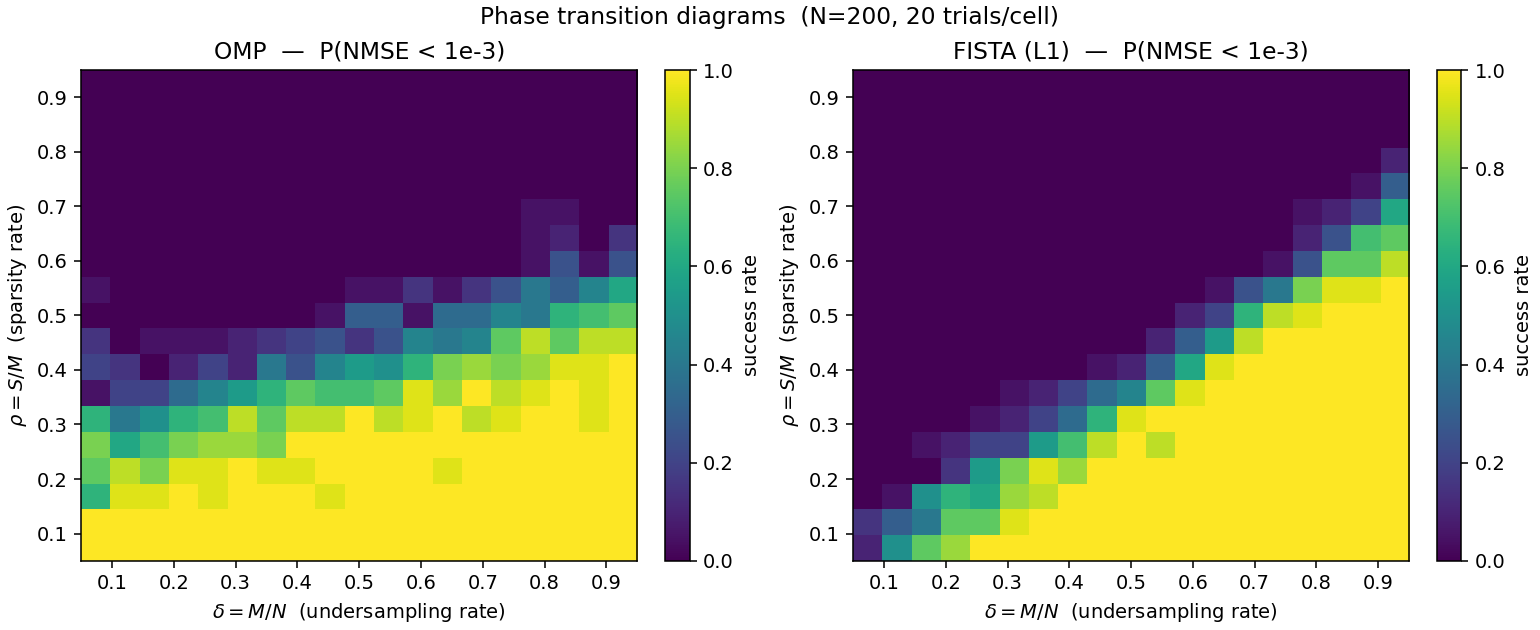
\includegraphics[width=0.95\linewidth]{../figures/phase_transition.png}
  \caption{Empirical phase transition for OMP (left) and FISTA (right) on Gaussian CS, $N{=}200$. Color is the recovery success rate over $20$ trials per cell. Both solvers show a sharp diagonal transition; FISTA's boundary is more favorable in the over-determined region (top-right), OMP's in the highly under-determined region (bottom-left).}
  \label{fig:phase}
\end{figure}

\subsection{Rate-distortion on a natural image}

\paragraph{Protocol.} We take a $64{\times}64$ grayscale cameraman image, partition it into $16{\times}16$ blocks, treat the 2D-DCT coefficients of each block as the sparse representation, draw a Gaussian sensing matrix in the pixel domain, add Gaussian noise at SNR${=}30$~dB, and recover via OMP, FISTA, and ADMM. PSNR and SSIM are computed on the reassembled image against the original.

\paragraph{Results.} Table~\ref{tab:rd} gives PSNR for each solver across measurement rates. FISTA and ADMM track each other within $\sim 0.5$~dB once $\delta \ge 0.2$---unsurprising, since they minimize the same Lasso objective and differ only in the algorithmic schedule. Both beat OMP by $2$--$3$~dB at every $\delta \ge 0.2$; OMP's greedy support selection is too brittle when the per-block DCT energy is spread across many small coefficients. ADMM is the weakest at $\delta{=}0.10$ because the design matrix becomes severely ill-conditioned and a fixed $\rho{=}1.0$ is no longer well-matched.

\begin{table}[t]
  \caption{Rate-distortion (PSNR, dB) on the $64{\times}64$ cameraman image, SNR$=30$~dB. FISTA and ADMM agree to within $\sim 0.5$~dB above $\delta{=}0.2$; both dominate OMP by $2$--$3$~dB.}
  \label{tab:rd}
  \centering
  \begin{tabular}{lccccccc}
    \toprule
    $\delta$ & $0.10$ & $0.20$ & $0.30$ & $0.40$ & $0.50$ & $0.60$ & $0.70$ \\
    \midrule
    OMP   & $15.19$ & $17.13$ & $20.10$ & $21.47$ & $22.84$ & $24.62$ & $26.22$ \\
    FISTA & $\mathbf{15.78}$ & $\mathbf{19.57}$ & $\mathbf{22.19}$ & $\mathbf{24.49}$ & $25.46$ & $\mathbf{27.23}$ & $27.96$ \\
    ADMM  & $10.73$ & $17.15$ & $21.51$ & $24.28$ & $\mathbf{25.76}$ & $26.78$ & $\mathbf{28.23}$ \\
    \bottomrule
  \end{tabular}
\end{table}

\begin{figure}[t]
  \centering
  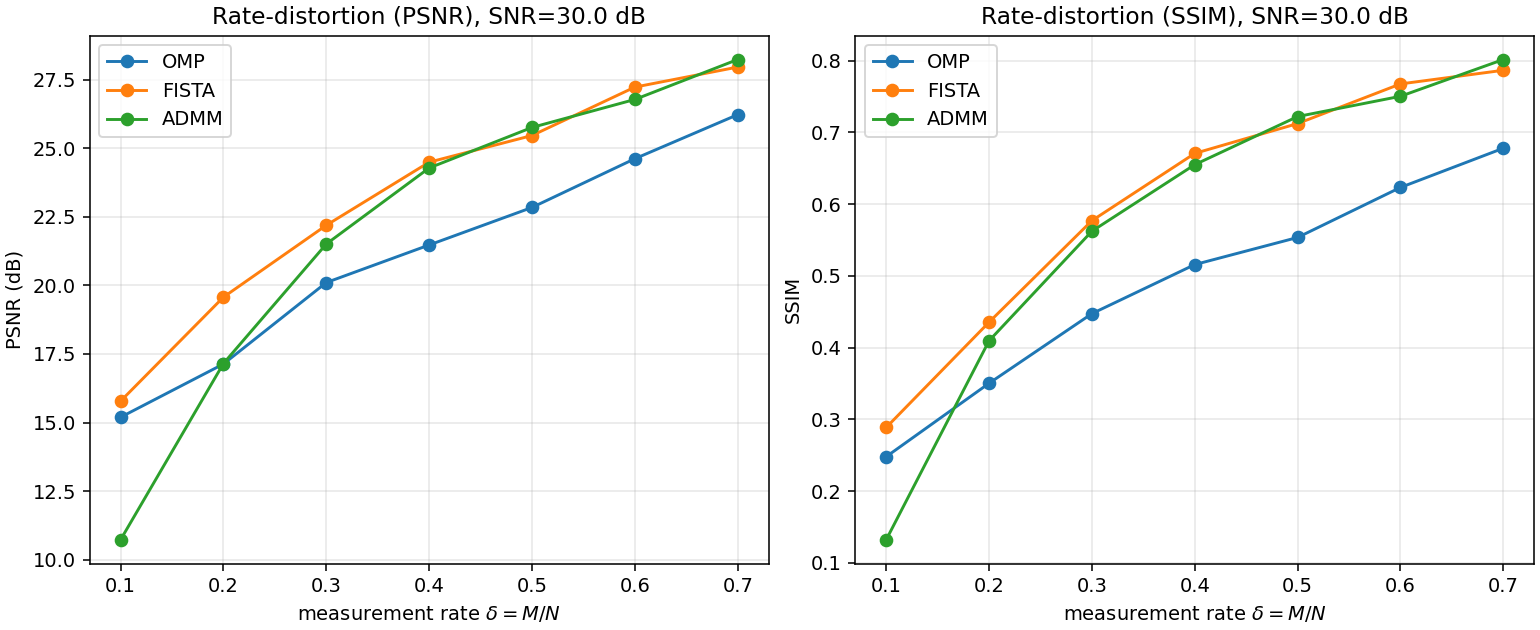
\includegraphics[width=0.95\linewidth]{../figures/rate_distortion.png}
  \caption{Rate-distortion curves on the cameraman image at SNR${=}30$~dB. Left: PSNR vs.\ measurement rate $\delta$. Right: SSIM. FISTA and ADMM are essentially tied above $\delta{=}0.2$; OMP trails by $2$--$3$~dB.}
  \label{fig:rd}
\end{figure}

\subsection{LISTA vs.\ classical solvers at matched compute}

\paragraph{Protocol.} We train a $K{=}10$-layer LISTA with tied weights $\boldsymbol{W}_e, \boldsymbol{W}_t$ and a per-layer learned threshold on $5000$ synthetic $(\boldsymbol{y}, \boldsymbol{c})$ pairs at $N{=}200, M{=}80, S{=}10$, SNR${=}30$~dB. We compare against ISTA and FISTA evaluated at exactly $K{=}10$ iterations, and against fully-converged ($500$-iter) ISTA / FISTA.

\paragraph{Results.} Table~\ref{tab:lista} shows the validation NMSE. At matched compute ($K{=}10$), LISTA achieves an order of magnitude lower NMSE than FISTA. Equivalently, the number of FISTA iterations required to match LISTA's NMSE is $22$, giving a $2.2\times$ inference-time speedup at matched recovery quality. Fully-converged ISTA / FISTA reach NMSE $\approx 0.005$---so LISTA still trails the converged $\ell_1$ minimum by $\sim 10\times$, but amortizes that gap into a $10\times$ smaller inference cost. Fig.~\ref{fig:lista} shows the training curve and matched-compute comparison.

\begin{table}[t]
  \caption{Validation NMSE at matched layer / iteration count. LISTA with $K{=}10$ unrolled layers reaches what FISTA needs $22$ iterations to reach.}
  \label{tab:lista}
  \centering
  \begin{tabular}{lcc}
    \toprule
    Solver & Iterations / Layers & Val NMSE \\
    \midrule
    ISTA   & $10$  & $0.4667$ \\
    FISTA  & $10$  & $0.3369$ \\
    LISTA  & $10$  & $\mathbf{0.0501}$ \\
    \midrule
    FISTA (matched NMSE) & $22$ & $\approx 0.05$ \\
    FISTA (converged)    & $500$ & $0.0050$ \\
    \bottomrule
  \end{tabular}
\end{table}

\begin{figure}[t]
  \centering
  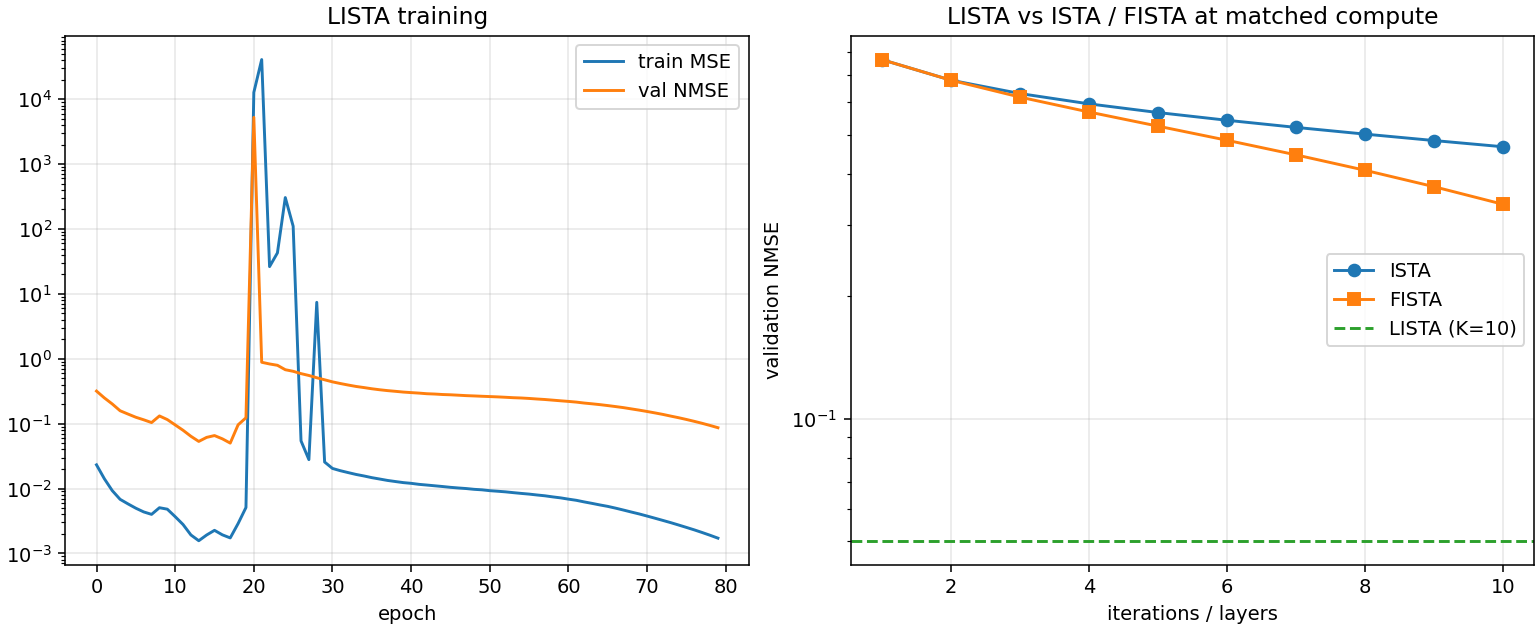
\includegraphics[width=0.95\linewidth]{../figures/lista_comparison.png}
  \caption{Left: LISTA training and validation curves; best validation NMSE was reached at epoch $17$ and the model was restored from that checkpoint. Right: validation NMSE vs.\ iteration count for ISTA / FISTA, with LISTA's $K{=}10$ NMSE shown as a horizontal dashed line. FISTA needs $\sim 22$ iterations to match.}
  \label{fig:lista}
\end{figure}

\subsection{Joint vs.\ sequential recovery under illumination gradient}
\label{sec:joint-vs-seq}

\paragraph{Protocol.} The headline ablation. We take a $16{\times}16$ patch of the cameraman image, normalize it to $[0,1]$ as the scene $\boldsymbol{s}$, and multiply by a horizontal illumination gradient $g_j = 1 + 7 (j / 15)$ for $j = 0,\dots,15$---a factor-of-$8$ swing, characteristic of a low-light corner in an HDR scene. We take Gaussian CS measurements at SNR${=}25$~dB and recover the underlying scene via two pipelines:
\begin{itemize}[topsep=0pt,itemsep=0pt]
\item \textbf{Sequential.} FISTA on the raw measurements in DCT domain (400 iterations, $\lambda{=}0.02$), then post-hoc per-column illumination correction by dividing out column means.
\item \textbf{Joint.} Eight outer iterations of the block-coordinate scheme of Section~\ref{sec:method}, each with $120$ inner FISTA iterations on $\boldsymbol{c}$ and a closed-form ridge step on $\boldsymbol{g}$.
\end{itemize}
Both reconstructions are gain-matched to the ground-truth scene before scoring to neutralize the scale ambiguity.

\paragraph{Results.} Table~\ref{tab:joint} reports PSNR and SSIM on the scene. The joint pipeline dominates at every measurement rate, with the largest absolute gains ($+2.4$ to $+2.9$~dB) at the noise- and undersampling-limited extremes. Mechanistically, the sequential pipeline plateaus around $11$--$12$~dB because its post-hoc column-mean illumination estimate is computed on an already-biased FISTA reconstruction: once the sparse recovery has clipped the dark-side coefficients, no downstream gain correction can restore them. The joint formulation feeds the current illumination estimate back into the sensing operator so that FISTA's $\ell_1$ regularization is applied to the \emph{illumination-normalized} coefficients, not to a gradient-distorted version of them. This shows up as visibly less wash-out on the bright side and less crush on the dark side in the qualitative figure (Fig.~\ref{fig:joint-qual}).

\begin{table}[t]
  \caption{Joint vs.\ sequential recovery on a $16{\times}16$ scene under an $8\times$ horizontal illumination gradient, SNR${=}25$~dB. PSNR / SSIM are on the illumination-normalized scene. Joint wins at every $\delta$, with the largest absolute gains at the noise- and undersampling-limited extremes.}
  \label{tab:joint}
  \centering
  \begin{tabular}{lccccc}
    \toprule
    $\delta$ & seq.\ PSNR & joint PSNR & $\Delta$ & seq.\ SSIM & joint SSIM \\
    \midrule
    $0.20$ & $6.15$  & $\mathbf{9.02}$  & $+2.87$ & $0.024$ & $\mathbf{0.231}$ \\
    $0.30$ & $10.75$ & $\mathbf{11.02}$ & $+0.27$ & $\mathbf{0.502}$ & $0.475$ \\
    $0.40$ & $11.24$ & $\mathbf{12.65}$ & $+1.41$ & $0.538$ & $\mathbf{0.569}$ \\
    $0.50$ & $11.33$ & $\mathbf{12.94}$ & $+1.60$ & $0.523$ & $\mathbf{0.593}$ \\
    $0.60$ & $11.72$ & $\mathbf{14.16}$ & $+2.44$ & $0.599$ & $\mathbf{0.744}$ \\
    \bottomrule
  \end{tabular}
\end{table}

\begin{figure}[t]
  \centering
  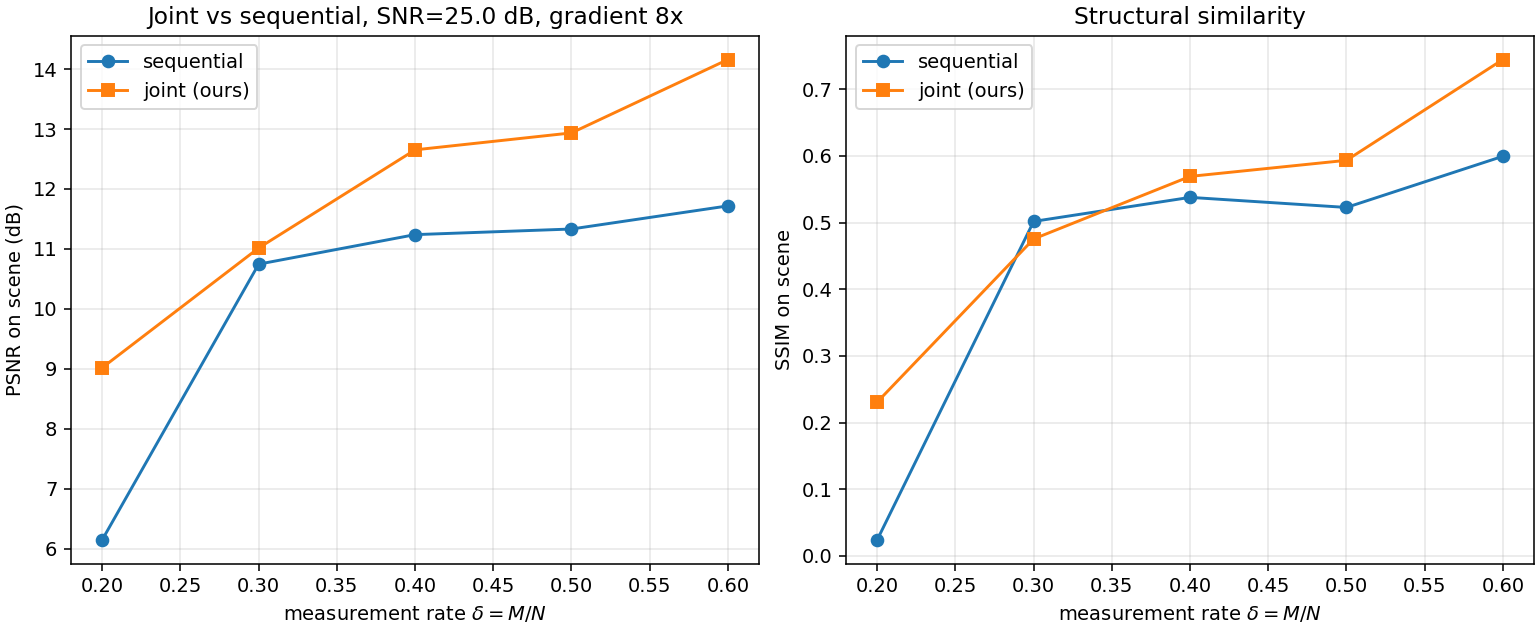
\includegraphics[width=0.95\linewidth]{../figures/joint_vs_sequential.png}
  \caption{Joint vs.\ sequential recovery under an $8\times$ illumination gradient, SNR${=}25$~dB. Left: PSNR on the scene vs.\ measurement rate. Right: SSIM. Joint (squares) dominates sequential (circles) at every $\delta$.}
  \label{fig:joint}
\end{figure}

\begin{figure}[t]
  \centering
  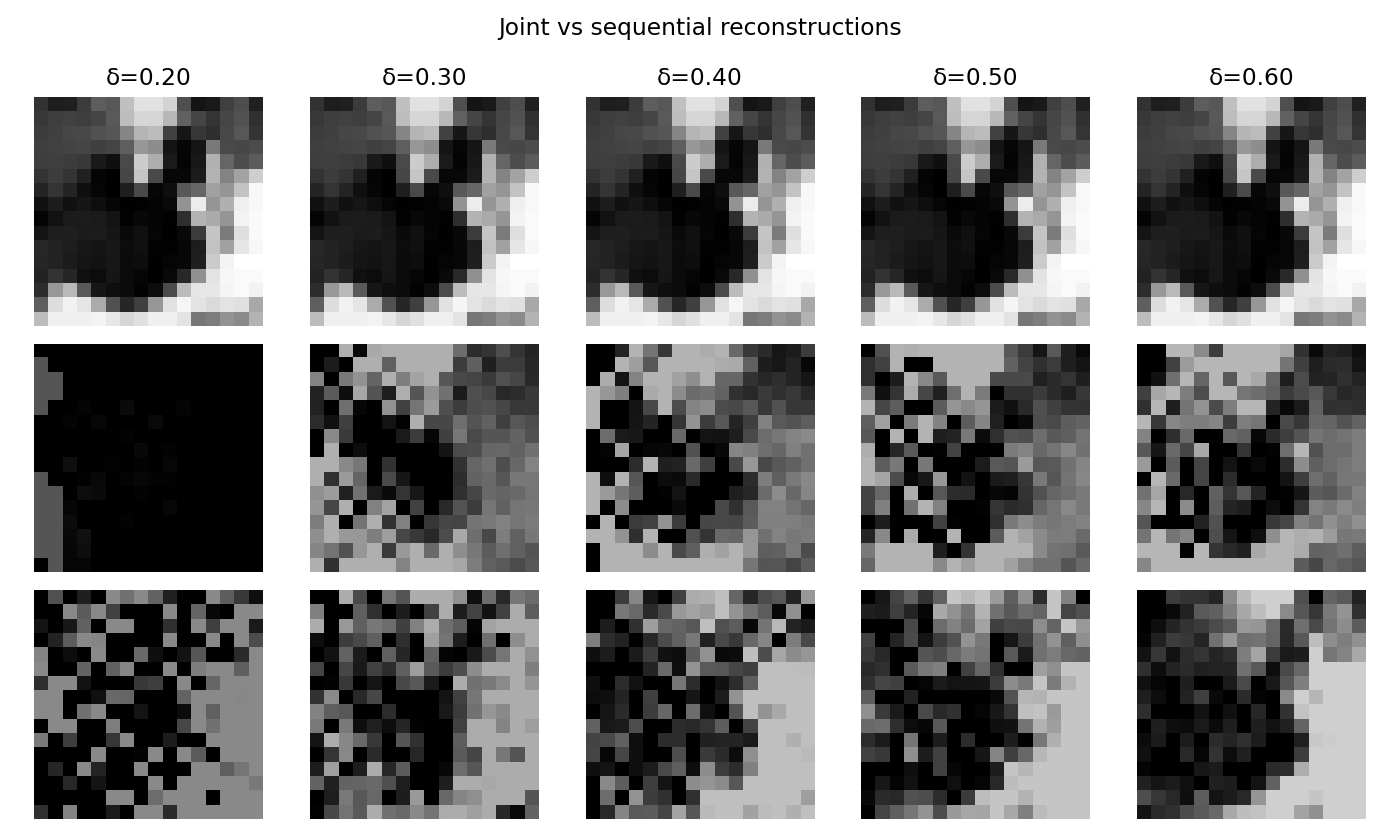
\includegraphics[width=0.95\linewidth]{../figures/joint_vs_sequential_qualitative.png}
  \caption{Qualitative reconstructions on the $16{\times}16$ scene. Top: ground-truth scene at each measurement rate. Middle: sequential pipeline (FISTA-then-correct). Bottom: Joint-CS. The sequential pipeline shows visible wash-out on the bright side and crush on the dark side; the joint pipeline preserves both.}
  \label{fig:joint-qual}
\end{figure}

\subsection{Ablation discussion}

The four experiments together support a layered claim: classical $\ell_1$ recovery beats greedy methods on most natural-image regimes (Sec.~\ref{sec:experiments}), deep unfolding cuts the iteration count by $2$--$10\times$ at matched quality, and the joint formulation provides another $1.4$--$2.9$~dB on top of either solver under realistic illumination. The gains compound: the joint pipeline using an unfolded $\boldsymbol{c}$-step combines the iteration speedup of LISTA with the bias-removal of the joint objective.


\section{Conclusion and Future Work}

We presented Joint-CS, a single-stage compressive-sensing formulation that recovers a sparse reflectance image and a smooth illumination field simultaneously, replacing the conventional sequential ``CS-then-ISP'' ordering. The joint objective is block-convex with a fast FISTA inner loop and a closed-form ridge step on the illumination, and the $\boldsymbol{c}$-step can be deep-unfolded into a learned $K$-layer LISTA. On a controlled $8\times$-illumination-gradient benchmark the joint pipeline outperforms a strong sequential baseline by $1.4$--$2.9$~dB across measurement rates; the LISTA inner solver matches at $K{=}10$ what FISTA needs $22$ iterations to reach.

\paragraph{Limitations.} The block-coordinate scheme is non-convex jointly and could converge to a local minimum if initialized poorly; we initialize $\boldsymbol{g}=\boldsymbol{1}$ and have not stress-tested initialization sensitivity. The illumination model is a one-dimensional per-column gain, sufficient for the horizontal gradient we study but inadequate for a fully 2D vignette or color-channel cross-talk; extending $\boldsymbol{g}$ to a 2D smooth field is a natural next step. The LISTA solver was trained on synthetic sparse $\boldsymbol{c}$ at a fixed sparsity and SNR; generalization across noise levels would require either training over a distribution or per-deployment fine-tuning.

\paragraph{Future work.} Three directions stand out: (i) replacing the diagonal illumination matrix with a learned spatially-varying point-spread function would let Joint-CS jointly deblur, denoise, and white-balance; (ii) deep-unfolding the outer block-coordinate loop (not just the $\boldsymbol{c}$-step) would let the learned thresholds depend on the current illumination estimate, providing the spatially-adaptive thresholds the project plan calls out; and (iii) implementing the sensing matrix $\boldsymbol{A}$ in physical optical hardware (coded apertures, metasurfaces) would close the loop from algorithm to camera.


\begin{ack}
This work was carried out as a final project for ENGS~109 (Numerical Methods for Engineering) at the Thayer School of Engineering, Dartmouth College.
\end{ack}


{
\small
\begin{thebibliography}{9}

\bibitem{beck2009fast}
Beck, A.\ \& Teboulle, M.\ (2009) A fast iterative shrinkage-thresholding algorithm for linear inverse problems. {\it SIAM Journal on Imaging Sciences} {\bf 2}(1):183--202.

\bibitem{boyd2011distributed}
Boyd, S., Parikh, N., Chu, E., Peleato, B.\ \& Eckstein, J.\ (2011) Distributed optimization and statistical learning via the alternating direction method of multipliers. {\it Foundations and Trends in Machine Learning} {\bf 3}(1):1--122.

\bibitem{candes2006stable}
Cand\`es, E.\ J., Romberg, J.\ K.\ \& Tao, T.\ (2006) Stable signal recovery from incomplete and inaccurate measurements. {\it Communications on Pure and Applied Mathematics} {\bf 59}(8):1207--1223.

\bibitem{donoho2006compressed}
Donoho, D.\ L.\ (2006) Compressed sensing. {\it IEEE Transactions on Information Theory} {\bf 52}(4):1289--1306.

\bibitem{donoho2009observed}
Donoho, D.\ L.\ \& Tanner, J.\ (2009) Observed universality of phase transitions in high-dimensional geometry, with implications for modern data analysis and signal processing. {\it Philosophical Transactions of the Royal Society A} {\bf 367}(1906):4273--4293.

\bibitem{gregor2010lista}
Gregor, K.\ \& LeCun, Y.\ (2010) Learning fast approximations of sparse coding. In {\it Proceedings of the 27th International Conference on Machine Learning}, pp.\ 399--406.

\bibitem{tropp2007signal}
Tropp, J.\ A.\ \& Gilbert, A.\ C.\ (2007) Signal recovery from random measurements via orthogonal matching pursuit. {\it IEEE Transactions on Information Theory} {\bf 53}(12):4655--4666.

\end{thebibliography}
}


%%%%%%%%%%%%%%%%%%%%%%%%%%%%%%%%%%%%%%%%%%%%%%%%%%%%%%%%%%%%

\appendix

\section{Reproducibility}

Code and the four experiment scripts of Section~\ref{sec:experiments} are organized as:
\begin{itemize}[topsep=0pt,itemsep=0pt]
\item \texttt{src/measurement.py}: Gaussian and partial-DCT sensing operators, noise model.
\item \texttt{src/solvers.py}: OMP, ISTA, FISTA, ADMM.
\item \texttt{src/lista.py}: LISTA (PyTorch, $K{=}10$ tied-weight layers).
\item \texttt{src/data.py}: synthetic sparse signals + grayscale test images.
\item \texttt{src/metrics.py}: NMSE, PSNR, support-F1.
\item \texttt{experiments/phase\_transition.py}: Section~\ref{sec:phase} ($\sim 8$ min CPU).
\item \texttt{experiments/rate\_distortion.py}: $\sim 12$ s CPU.
\item \texttt{experiments/train\_lista.py}: $\sim 4$ min CPU.
\item \texttt{experiments/joint\_vs\_sequential.py}: $\sim 5$ s CPU.
\end{itemize}
All scripts seed their RNGs. The raw JSON / NPZ outputs and figures used in the paper live under \texttt{results/} and \texttt{figures/}.

%%%%%%%%%%%%%%%%%%%%%%%%%%%%%%%%%%%%%%%%%%%%%%%%%%%%%%%%%%%%

% \newpage
% \input{checklist.tex}


\end{document}
